% Scalar instruction entry source: tools/generate_scalar_instruction_catalog.py.
\subsection{\texttt{OR}}
\label{sec:scalar-or}
\index{OR@\texttt{OR}}
\begin{sloppypar}\noindent\textbf{Purpose.} Bitwise OR.\end{sloppypar}\smallskip
\noindent\textbf{Syntax.}\par
\begin{lstlisting}[style=ptoscalarcode]
or SrcL, SrcR<{.sw,.uw,.not}><<<shamt>, ->RegDst
\end{lstlisting}
\noindent\textbf{Encoding.}\par
\noindent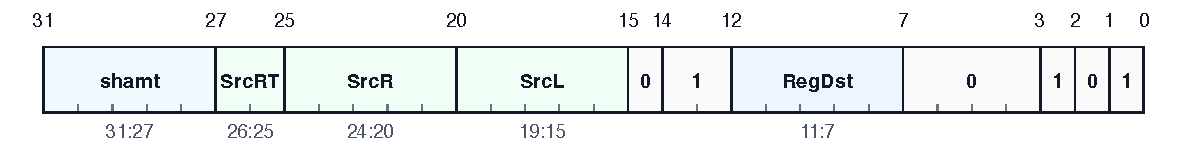
\includegraphics[width=\textwidth]{figs/encoding/scalar_instruction_entries/enc_or.pdf}\par\smallskip
\begin{description}[leftmargin=0.18\linewidth,style=nextline]
\item[Format] \texttt{L32} \texttt{32-bit} scalar word.
\item[Pattern] \texttt{.................011.....0000101}.
\end{description}
\noindent\textbf{Classification.}\par
\begin{description}[leftmargin=0.18\linewidth,style=nextline]
\item[Category] Integer ALU and Bit-Manipulation.
\item[Family] Arithmetic Operation 64bit.
\item[Execution class] \texttt{ALU}; uop\_kind=ALU.
\end{description}
\noindent\textbf{Operand fields.}\par
\begin{description}[leftmargin=0.18\linewidth,style=nextline]
\item[\texttt{RegDst}] Bits \texttt{11:7 (5b)}. 5-bit scalar destination register written by this instruction; X0 is hardwired to zero, so writes to X0 are ignored.
\item[\texttt{SrcL}] Bits \texttt{19:15 (5b)}. 5-bit scalar source register used as the left input operand.
\item[\texttt{SrcR}] Bits \texttt{24:20 (5b)}. 5-bit scalar source register used as the right input operand before any encoded modifier or shift is applied.
\item[\texttt{SrcRType}] Bits \texttt{26:25 (2b)}. 2-bit modifier for SrcR. It selects the encoded source form shown in the syntax, such as signed-word, unsigned-word, negated, or unmodified register input.
\item[\texttt{shamt}] Bits \texttt{31:27 (5b)}. 5-bit shift amount applied to the modified right operand before the ALU or address calculation uses it.
\end{description}
\noindent\textbf{Operation.}\par
\begin{lstlisting}[style=ptoscalarcode]
lhs = Read(SrcL)
rhs = Read(SrcR)  // apply modifiers/shift as encoded
result = lhs | rhs
Write(RegDst, result)
\end{lstlisting}
\Needspace{0.08\textheight}
